\documentclass{sig-alternate-10pt}

\usepackage{amsmath}
\usepackage{amssymb}
\usepackage{xcolor}
\usepackage{times}
\usepackage{xspace}
\usepackage{listings}

\newcommand{\todo}[1]{\textcolor{red}{[TODO: #1]}}
\newcommand{\ratul}[1]{\textcolor{blue}{[ratul: #1]}}
\newcommand{\ryan}[1]{\textcolor{green}{[ryan: #1]}}

\newcommand{\sysname}{{\small \sf Propane}\xspace}

\newcommand{\para}[1]{\paragraph*{\textbf{#1}}}

\newcommand{\path}[2]{ #1 \mapsto \ensuremath{#2} }

\begin{document}

\special{papersize=8.5in,11in}
\setlength{\pdfpageheight}{\paperheight}
\setlength{\pdfpagewidth}{\paperwidth}

\title{Programming Distributed Control Planes}
\author{Paper \#XXX}

\maketitle

%\category{CR-number}{subcategory}{third-level}
%% general terms are not compulsory anymore,
%% you may leave them out
%\terms
%term1, term2
%\keywords
%keyword1, keyword2

\section{Introduction}
\label{sec:introduction}

It is well-known that network configuration is highly error
prone and that such errors can lead to costly network
downtime~\cite{mahajan+:bgp-misconfiguration,feamster+:rcc,batfish}.
For instance, a recent misconfiguration led to an hour-long, nation-wide outage for Time Warner's backbone network~\cite{time-warner}; and a major BGP-related incident makes international news every few months~\cite{bgpmon}.

%For instance, in the context of BGP, Mahajan~~\cite{mahajan+:bgp-misconfiguration}
%estimated that 200-1200 prefixes suffered from
%misconfiguration each day and that close to 3 in 4 of all
%new prefix advertisements were the result of misconfiguration.
%Moreover, these misconfigurations sometimes cause significant network downtime for
%individual networks~\cite{time-warner} or even broader internet connectivity problems~\cite{routing-instability,mahajan+:bgp-misconfiguration}.
%\dpw{Note that \cite{time-warner} and I am not sure about the specifics of the problem there
%or what exactly was misconfigured.  It is also unclear if our language really helps with the
%``broader internet connectivity problems'' however, I thought that adding some specific examples
%would help make the intro more compelling.  Feel free to rewrite.}

One reason for network configuration being onerous is that device configuration languages are low-level and several configuration elements must be kept consistent (e.g., interface addresses) for the device to behave as intended.

Another, more fundamental reason is the semantic mismatch between the intended high-level
policies and the low-level device-by-device configurations.  In particular,
many policies involve network-wide properties---prefer a certain neighbor,
never announce a particular destination externally,
use a particular path only if another fails---but configurations describe the behavior of
individual devices.
%
Operators must manually decompose network-wide policy into device-level behaviors, such that their interactions satisfy the high-level objectives.
%
Ensuring policy-compliance through this manual decomposition is challenging under normal
circumstances and even more so in the face of failures. Some decompositions that work correctly
in failure-free environments, violate key constraints when failures occur.
%
As a result, many network configuration problems are only revealed after failures~\cite{batfish},
sometimes making a bad situation worse.

To reduce configuration errors, many practitioners have a adopted a template-based
approach~\cite{hatch,thwack}, in which common configuration patterns are captured as parameterized templates.
 While templates help ensure certain kinds of consistency across devices, they do not
bridge the
semantic divide between network policies and device-level configuration.
They do not provide fundamentally different abstractions
from existing configuration languages.

Software-defined networking (SDN) and its abstractions 
are, in part, the research
community's response to the difficulty of maintaining policy
compliance through distributed interaction of individual
devices~\cite{sdn-languages}. Indeed, instead of organizing networks
around a distributed collection of devices that compute forwarding tables through
mutual interactions, the devices are told how to
forward packets by a centralized controller. The controller is responsible for ensuring that the
paths taken are compliant with operator specifications.
%Researchers
%have developed increasingly sophisticated languages that let operators
%specify desirable network paths~\cite{x,y,z} which are then translated
%to forwarding tables at runtime.

The centralized control planes of SDN, however, are not a panacea.
%
They require careful design and engineering to be robust to failures at scale---one must ensure that all devices can communicate with the controller at all times, even under arbitrary combinations of failure~\cite{x,y,z}. To address this challenge, many researchers are beginning to explore
multi-controller networks, with interacting controllers, thus bringing back distributed
control planes~\cite{x,y,z} and their current programming difficulties.  However, academic
language design and implementation efforts have not kept pace.  For instance, work on
experimental SDN languages
such as Frenetic~\cite{frenetic}, Flowlog~\cite{flowlog}, Vericon~\cite{vericon}, Merlin~\cite{merlin}, NetKAT~\cite{netkat}, and Kinetic~\cite{kinetic}, to
name a few, has not yet shown how to implement fault tolerant
multi-controller systems that support their abstractions efficiently.

In this paper, we ask if it is possible to program distributed control planes using network-wide policies.
Operators should be able to directly express network-wide policies, which are automatically decomposed into individual device configurations. The resulting forwarding behavior, which emerges through device interactions, must be policy-compliant under all possible failures.
If successful, this approach would combine easy programmability of centralized control planes and failure robustness of distributed control planes.
%
More pragmatically, it would help many networks that, for the foreseeable future, will continue to use a distributed control plane, due to the difficulty of migrating to SDN or the inherent scalability and failure-robustness of distributed control.

Through \sysname, our system that includes a language and a compiler, we demonstrate the feasibility of programming distributed control planes. We focus on BGP, a common and highly flexible way to implement distributed control planes, and show how to automatically generate router BGP configurations from network-wide policies.

We face two challenges in designing \sysname that differ from designing a system for programming data planes~\cite{x,y,z}. The first is policy specification itself---specifying network {\em policies} is different from specifying network {\em paths}.
%
The specification must compactly capture behavior under all possible failures. Since there is no controller at runtime, the routers must be programmed ahead of time, based on the specification, to handle failures.
%
Further, many policies naturally under-specify paths (e.g., "prefer paying neighbors" is not a concrete path).
%
\sysname addresses this specification challenge by allowing operators to express {\em path preferences}, where preference describes a set of valid paths and less-preferred options are taken only when a higher-preference options are unavailable.

The direct nature of \sysname specifications brings up the second challenge, of compiling them to router configurations.  We must compute the sets of paths represented by the intersection of multiple preferences and topology, compute which ones can be honored under a given failure scenario, and ensure policy compliance under all possible failure cases. We handle this challenge by compactly capturing policy and topology in a {\em product graph} and developing efficient algorithms that operate on this graph.

We evaluate \sysname by using it to encode policies of real backbone and data center networks.

\todo{new intro is not complete}



\section{Background on BGP}
\label{sec:background}

%Our work focuses on BGP as it is the most common and flexible way to implement distributed control planes today. In this section, we provide relevant background on BGP.

BGP is a path-vector routing protocol that connects autonomous systems (ASes). An AS has one or more routers managed by the same administrative entity. ASes exchange routing announcements with their neighbors. Each announcement has a destination IP prefix and some attributes (see below), and it indicates that the sending AS is willing to carry traffic destined to that prefix from the receiving AS. Traffic flows in the opposite direction, from announcement receivers to senders.

When a route announcement is received by an AS, it is processed by custom import filters that may drop the announcement or modify some attributes. If multiple announcements for the same prefix survive import filters, the router selects the best one based on local policy (see below). This route is then used to send traffic to the destination. It is also advertised to the neighbors, after processing through neighbor-specific export filters that may stop the announcement or modify some attributes.

All routing announcements are accompanied by an AS-path attribute that reflects the sequence of ASes that the announcement has traversed thus far. While the AS-path attribute has a global meaning, some attributes are meaningful only within an AS or between neighboring ASes.  One such attribute is a list of community strings. ASes use such strings to color routes on different criteria (e.g., ``entered on West Coast'') and then use the color later in the routing process.  Communities are also used to signal to neighbors how they should handle an announcement (e.g., do not export it further). Another non-global attribute is the multi-exit discriminator (MED). It is used when an AS has multiple links to a neighboring AS.  Its (numeric) values signal to the neighbor how this AS prefers to receive traffic among those links.

The route selection process assigns a {\em local preference} to each
route that survives the import filters. Routes with higher local
preference are preferred. Among routes with the same local preference,
other factors such as AS path length, MEDs, and internal routing cost, are considered in order. Because it is considered first during route selection, local preference is highly influential, and ASes may assign this preference based on any aspect of the route. A common practice is to assign it based on the commercial relationship with the neighbor. For instance, an AS may prefer in order customer ASes (which pay money), peer ASes (with free exchange of traffic), and provider ASes (which charge money for traffic).

In implementing their policy, each network operator assumes that
neighboring ASes correctly implement BGP and honor contracts related
to MEDs and communities. \sysname makes the same assumption when
deriving BGP configurations for a network.

The combination of arbitrary import and export filters and route selection policies at individual routers make BGP a highly flexible routing protocol. That flexibility, however, comes at the cost of it being difficult to configure correctly, as we explain next.

\section{Motivation and Propane overview}
\label{sec:motivation}

%We motivate our work by describing the current practice in network
%configuration. In traditional networks with distributed control planes, the operators' goal is to generate the configuration of individual devices based on their desired policy. This configuration dictates the behavior of a device, how it exchanges routing information with neighbors and how it filters and ranks that information. The collective behavior of the devices should implement the desired policy.
%
%Device configuration languages are low-level and indirect. For instance, instead of allowing operators to express directly the paths they want through the network, they require operators to specify metrics that result in those paths; instead of allowing operators to express directly the types of traffic to not carry through the network, they require operators to select and program an appropriate filtering mechanism (e.g., BGP import or export filters, null routing,  access control lists) and instantiate it on topologically appropriate devices; instead of allowing operators to directly specify that they prefer BGP neighbors in a certain order, they require operators to program local preferences and multi-exit discriminators (MED) at each router and ensure that the numbers are consistent across routers.
%
%In many networks today, device configurations are generated manually by operators, without the support of many automated tools. It is easy to see the problems with this approach, such as typos, inconsistency across devices, and no guarantees of policy compliance.
%
%To reduce such problems, some networks use a template-based approach. Configuration templates abstract certain constants into variables (e.g., instead of concrete community value, they may contain a variable {\small \sf{\$$BadNeighbor$)}} and may use a device vendor-neutral syntax. Operators manually generate the templates and use tools to translate them into device configuration, by replacing variables with appropriate constants using a database of network information.
%
% %and replacing vendor-neutral constructs with their vendor-specific counterparts.
%
%%In practice, most networks use a hybrid of templates and manual generation of device configuration. Templates are used for standardized and common configuration elements across devices and the result is manually tweaked to obtain the exact desired network behavior.
%
%While templates avoids some pitfalls of the fully manual approach, they too are far from ideal. The fundamental issue is the semantic mismatch between desired policies and the level of abstraction of templates. While many policies are network-wide (e.g., prefer customer networks, or never announce a route to a certain prefix to external neighbors), templates are device-level. Operators must still manually decompose network-wide policies into device-level policies that can produce the desired network-wide behavior.
%This decomposition is not always straightforward and ensuring policy-compliance can be hard, especially in the face of failures. We illustrate this point using two examples based on policies that we have seen in practice and we demonstrate the ease with which the
%examples are described using our new language \sysname.

In networks with distributed control planes, the operators today generate the configuration of individual devices based on intended policy. Whether this task is done fully manually or with the aid of templates, the challenge is to decompose network-wide policies 
%(e.g., prefer customer networks, or never announce a route to a certain prefix to external neighbors), 
into device-level policies that collectively produce the intended behavior.
This decomposition is not always straightforward and ensuring policy-compliance can be hard, especially in the face of failures. We illustrate this point using two examples based on policies that we have seen in practice. We also demonstrate the ease with which the
policies can be specified using our new language \sysname. The next section describes how to automatically compile this specification to device-level policies.

\begin{figure}[t!]
\centering
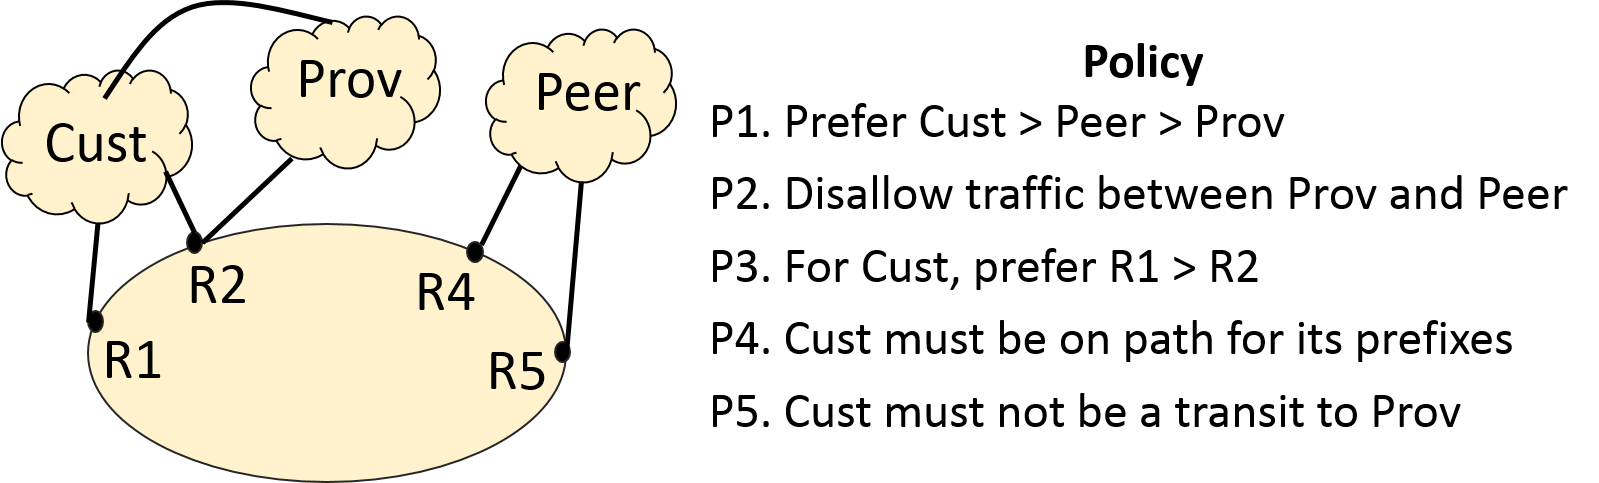
\includegraphics[width=\columnwidth]{figures/example1}
\caption{Creating router-level policies is difficult.}
\label{fig:example1}
\end{figure}


\subsection{Example 1:  The Backbone}

Consider the backbone network in Figure~\ref{fig:example1}. It has three neighbors, a customer $Cust$ , a peer $Peer$, and a provider $Prov$. The policy of this network is shown on the right. It prefers the neighbors in a certain order ($P1$) and does not want to act as a transit between Peer and Prov ($P2$). It prefers to exchange traffic with Cust over $R1$ rather than $R2$ because $R1$ is a cheaper ($P3$). To guard against another AS "hijacking" prefixes owned by Cust, it only sends traffic to them if Cust is on the AS path ($P4$). Finally, to guard against Cust accidentally becoming a transit for Prov, it does not use Cust for traffic that will later traverse Prov ($P5$).

To correctly implement this policy, the operators must compute and assign local preferences such that preferences at Cust-facing interfaces $>$ Peer-facing interfaces $>$ Prov-facing interfaces. At the same time, the preference at $R2$'s Cust-facing interface should be lower than that at $R1$, but higher than that at Prov-facing interface. To fully realize $P2$, MEDs will have to be appropriately configured as well. To implement $P3$ and $P4$, the operators may assign communities that indicate where a certain routing announcement entered the network. Then, R4 must not announce to $Peer$ routes that have communities that correspond to the R2-prov link but must announce communities for the $R2$-Cust and $R1$-Cust links. Finally, to implement $P4$ and $P5$, the operators will have to compute and configure appropriate prefix- and AS-path-based filters at each router.

We can now see how devising correct configuration for real, larger networks will quickly become a nightmare. The networks will have many neighbors across multiple classes of commercial relationships, differing numbers of links per neighbor, along with several region-, neighbor- or prefix-based exceptions to the default behavior. Templates help by keeping preference and community values consistent across routers, but operators must still do much of the conceptually difficult work manually.
%, in coming up with the templates themselves.

\begin{figure}[t!]
\centering
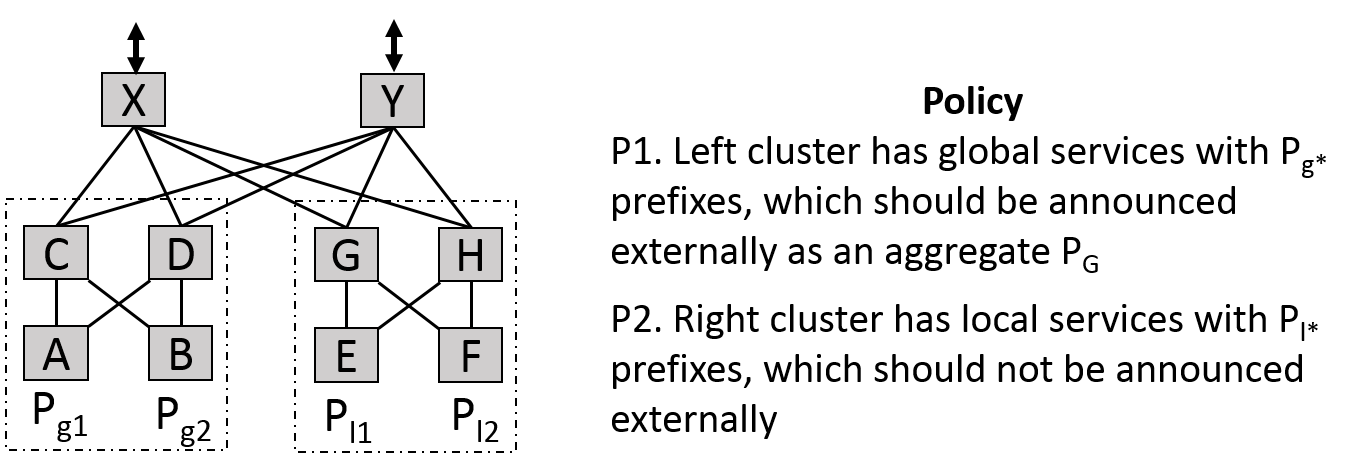
\includegraphics[width=\columnwidth]{figures/example2}
\caption{Policy-compliance under failures is difficult.}
\label{fig:example2}
\end{figure}

\para{The Backbone in \sysname}
\sysname simplifies network configuration by allowing users to
specify end-to-end forwarding paths and associating them with
appropriate prefixes.  The \sysname compiler handles the task of
generating low-level BGP configurations consistent with the user's
specifications.  It automatically synthesizes
import-export filters, local preferences, MED attributes, and community tags
to ensure policy compliance under all possible failure scenarios.

In general, \sysname specifications are written modularly via a series
of user declarations.
%These definitions allow users to express the three
%major elements of any \sysname specification:  \emph{prefixes},
%\emph{paths} and \emph{policies}.
For example, to begin specification of the backbone
network, we first express the idea that for routes leading to our customer,
we prefer using $R_1$ over $R_2$ (Policy P3 from Figure~\ref{fig:example1}):
\begin{lstlisting}[mathescape=true]
define ExitCust = $exit(R_1 \gg R_2)$
\end{lstlisting}
The  statement above defines a set of \emph{ranked paths}, which includes
all paths (and only those paths) that \cd{exit}
our network
through either router $R_1$ or $R_2$.  The paths that exit through $R_1$
are preferred ($\gg$) to the paths that exit through $R_2$.

To associate ranked paths with
one or more prefixes, we must define a \sysname \emph{policy}.
Within a policy, statements with the form $\path{x}{p}$
associate the prefixes defined by the predicate $x$ with the set of
ranked paths defined by the path expression $p$.
For instance, in the following code, ranked paths are associated with
the customer prefixes ($C_{pfx}$), the internal prefixes ($I_{pfx}$),
and all other prefixes (\cd{true}).\footnote{Policy statements are processed in
order with earlier policy statements taking precedence over later
policy statements.  Hence, when the prefix predicate \cd{true} follows
statements involving $C_{pfx}$ and $I_{pfx}$, it is interpreted as
$\cd{true} \AND \NOT C_{pfx} \AND \NOT I_{pfx}$.}

\begin{lstlisting}[mathescape=true]
define Routing = {
    $\path{C_{pfx}}{ExitCust \gg end(Cust)}$
    $\path{I_{pfx}}{end(in)}$
    $\path{true}{ExitCust \gg exit(Peer) \gg exit(Prov)}$
}
\end{lstlisting}

Line 2 of the policy above
defines the paths that exit our network to customer prefixes ---
\cd{ExitCust} defines paths through $R_1$ and $R_2$ and in the event
that connections to the customer through both of those routers fail,
a backup route ($end(Cust)$) is defined that admits traffic to go through
any path that ends at the customer.
Line 3 states that traffic for internal prefixes must end in our network, and is otherwise unconstrained.  The special keyword \cd{in} represents any location
inside the user's network whereas the keyword \cd{out} represents any location
outside the user's network.
Line 4 applies to any other traffic, and allows for any routes that leave through a peer with a preference for customers over peers over providers. To summarize our progress so far, the \cd{Routing} policy
implements (P1), (P3) and (P4) from Figure~\ref{fig:example1}

Since, routing still allows transit traffic (e.g., traffic can enter from \textit{Peer} and leave through \textit{Prov}), we can define a new policy that
implements this restriction separately.

\begin{lstlisting}[mathescape=true]
define PP = Peer or Prov
define PPTransit = $enter(PP) \AND exit(PP)$
define CustTransit = $later(Cust) \AND later(Prov)$

define NoTransit = {
    $\path{true}{\neg PPTransit \AND \NOT CustTransit}$
}
\end{lstlisting}

The \textsf{NoTransit} constraint above ensures that requirements (P2) and (P5) are satisfied. In particular, it says that for any prefix, traffic should never both enter and exit the network from \textit{Peer} or \textit{Prov}. Similarly it prevents traffic from ever following paths that leave our network and later passing through both \textit{Prov} and \textit{Cust}.  To implement both \cd{Routing}
and \cd{NoTransit} simultaneously, we simply conjoin them:

\begin{lstlisting}[mathescape=true]
Routing $\AND$  NoTransit
\end{lstlisting}

\sysname will generate per-device import and export filters, local preferences,
MED attributes, and community tags to ensure that the policy is
implemented correctly under all failure scenarios.

\subsection{Example 2:  The Data Center}

If configuring policies for a fully functional network is difficult, doing so in a way that ensures policy compliance in the face of failures can be almost impossible. Consider the data center network in Figure~\ref{fig:example2} with routers organized as a fat tree and running BGP.\footnote{To scale and to simplify policy implementation, data center networks increasingly use BGP internally, with a private AS number per router~\cite{bgp-in-dc-rfc}.} The network has two clusters, one that hosts services that should be reachable globally and one that hosts that should be accessible only internally. This policy is enabled by using non-overlapping address space in the two clusters and ensuring that only the address space for the global services is announced externally. In addition, to reduce the number of prefixes that are announced externally, the global space is aggregated into one larger, less-specific prefix $P_G$. The semantics of aggregation in BGP is that the aggregate prefix is announced as long as the router has a path to even one sub-prefix.

The operator may decide that a simple way to implement the policy is to have X and Y: $i)$ not export externally what they hear from routers G and H since these routers border the cluster with local services; and $ii)$ announce what they hear from routers C and D and aggregate to $P_G$ if an announcement is subset of $P_G$. The appeal of this implementation is that X and Y do not need to be made aware of which prefixes are global versus local and IP address assignment can be done independently (e.g., new prefixes can be added to local services without updating router configurations).

However, this implementation is incorrect because it does not have the right behavior in the face of failures. Suppose links X--G and X--H fail. Then, X will hear announcements for $P_{l*}$ from C and D, having traversed from G and H to Y to C and D. Per policy implementation, X will start "leaking" these prefixes externally. Depending on the rationale for local services, this leak could impact security (e.g., if the services were sensitive) or availability (e.g., if the $P_{l*}$ prefixes are used for other services outside of the data center). This problem does not manifest without failures because then X has and prefers paths to $P_{l*}$ through G and H since they are shorter. A similar problem will happen if links Y--G and Y--H fail.
%\footnote{A different problem occurs when links X--C and X--D (or Y--C and Y--D) fail. X (Y) may stop announcing the global prefixes because they would be heard through G and H.}
Link failures in data centers are frequent and it is not uncommon to have multiple failed links at a given time~\cite{dc-failure-study}.

To avoid this problem, the operator may decide to disallow paths with "valleys," i.e., those that go up, down, and back up again. This safeguard can be implemented by $X$ and $Y$ rejecting paths through the other. However, that creates a different problem in the face of failures---an aggregation-induced blackhole~\cite{xx}. Suppose links D--A and X--C fail. Now, X will hear announcements for $P_{g2}$ from D and will thus announce the $P_G$ externally. This announcement will bring to X traffic for $P_{g1}$ as well, but because of valley-free filtering, X does not have a valid route for $P_{g1}$ and will thus drop all traffic to it.

Thus, we see that devising a configuration that ensures policy compliance in the face of failures is complex and error-prone. \sysname helps operators by implementing their high-level policy specification in a way that guarantees compliance under all failures if that is possible. Otherwise, it generates a compile-time error that informs them that the specification cannot be met. For aggregation, it will also provide a lower bound to operators on the number of failures under which aggregation will not result in blackholes.

\para{The Data Center in \sysname}
In our data center example,
there are primarily three main concerns:
(1) traffic for the prefix block allocated to each top-of-rack router must be able to reach that router,
(2) local services must not leak outside the datacenter, and
(3) aggregation must be performed on global prefixes to reduce churn
in the network.

\sysname allows us to decompose and specify each of these constraints in a modular fashion. The first constraint is about prefix ownership -- namely, that we only want traffic for certain prefixes to end up at a particular locations. The following definition captures this intent.

\begin{lstlisting}[mathescape=true]
define Ownership = {
    $\path{p_{g1}}{end(A)}$
    $\path{p_{g2}}{end(B)}$
    $\path{p_{l1}}{end(E)}$
    $\path{p_{l2}}{end(F)}$
}
\end{lstlisting}

In English: traffic for prefix $p_{g1}$ is only allowed to follow paths that
end at router A; traffic not matching $p_{g1}$, but which matches $p_{g2}$ must
end at router B; and so on.

To capture the second constraint, we can define another task for the core
routing policy:

\begin{lstlisting}[mathescape=true]
define Routing = {
    $\path{p_{g*}}{any}$
    $\path{p_{l*}}{\NOT enter(out)}$
    $\path{true}{exit(out)}$
}
\end{lstlisting}

The first line states that there is no restriction (\cd{any})
on how traffic must
traverse the network for global prefixes, aside from the default restriction
that traffic must not pass through the user's network and then loop
back on itself. This means traffic for
$p_{g*}$ may be sent either from other routers in the datacenter, or
from external ASes. The second line ensures that traffic for local
prefixes never enters the network from an outside location. This constraint
guarantees that the services remain reachable only to locations
internal to the data center.

As in the backbone example, we can combine these constraints
logically to specify the network-wide policy.
However, in addition to constraints on the shape of paths,
\sysname allows the operator to specify constraints on the BGP control plane.
For instance, a constraint on aggregation is included to ensure that
aggregation for $p_{agg}$ is performed from locations inside the network
to locations outside the network. \todo{Say more about aggregation here.
What prefixes are aggregated in to what blocks?  How is this defined?}

\begin{lstlisting}[mathescape=true]
Ownership $\wedge$ Routing $\wedge$ agg($p_{agg}$, $in \rightarrow out$)
\end{lstlisting}

As before, once \sysname compiles the policy, it is guaranteed to hold under
all possible failure scenarios. In addition, the system can check for
aggregate-induced black holes in the presence of up to $k$ failures.
\todo{Note:  Another comment about failure checking for black holes, which may
not be implemented yet.}


%\subsection{OLD -- Overview}
%\todo{this subsection can be deleted once we have captured everything in it}
%
%Sources of bugs we fix. (It seems like the main advantage of our approach is not just fixing bugs though - it is easily describing high-level intention).
%Perhaps the best way to do this is by going through a bunch of examples in section 2 and showing how you could easily introduce bugs:
%
%\begin{itemize}
%	\item Out of sync, or copy paste errors due to replicated configs (never an issue due to centralized control)
%	\item Correct filtering to ensure no undesired traffic can flow through the network (e.g., best practices, like an AS should filter customers for their prefix, are implemented automatically )
%	\item Failures can easily lead to unexpected behavior (e.g., a datacenter failure scenario w/instability.)
%	\item Trying to do anything interesting, like get backups correct is difficult (e.g., setting up aggregation wrong)
%	\item Related to the last point, things like aggregation can introduce black holes. We have the information needed to prevent this
%\end{itemize}
%
%
%Possible Examples:
%\begin{itemize}
%	\item Basic datacenter with spine preference
%	\item Simple AS that prefers customers over peers over providers
%	\item Combined internal backup routing with preference based entrance into the network using aggregation.
%	\item Something like cold potato routing
%\end{itemize}


\section{Propane}
\label{sec:propane}

Show how to solve examples from the previous section.



\section{Compilation}
\label{sec:compilation}





\subsection{Overview}

\begin{figure}[t!]
\centering
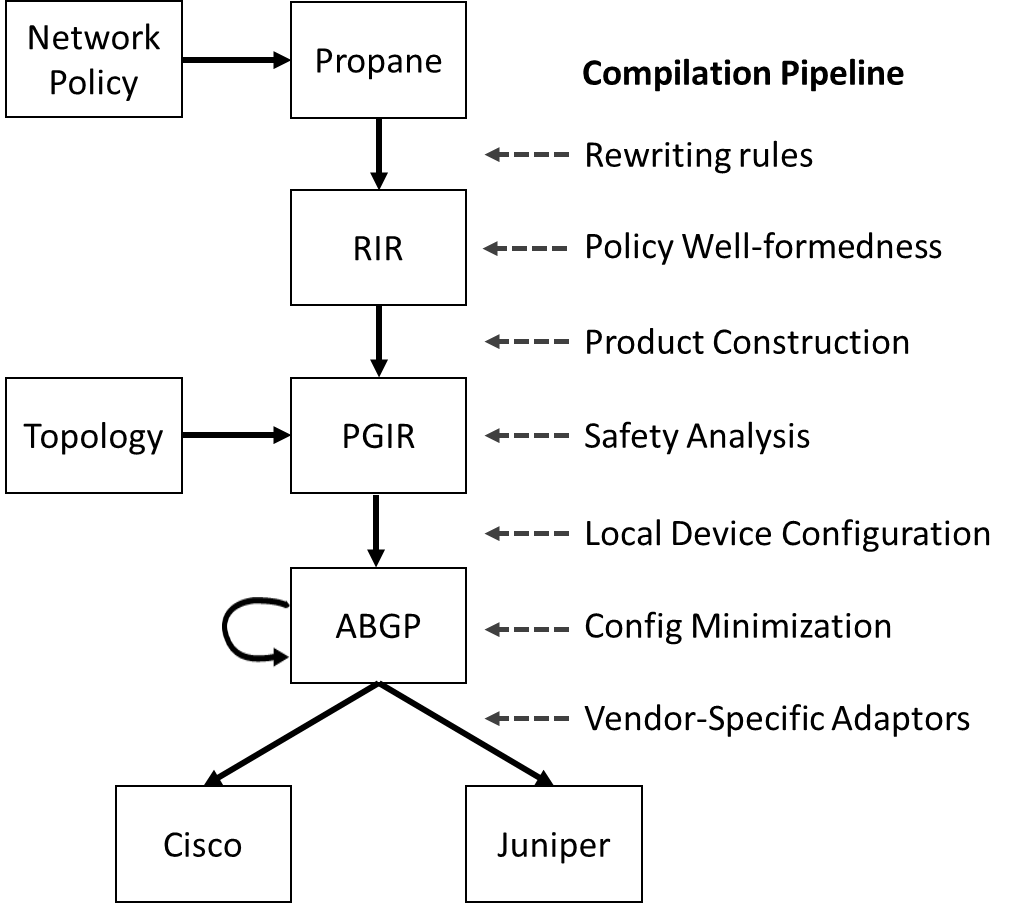
\includegraphics[width=\columnwidth]{figures/pipeline}
\caption{Compilation pipeline stages for Propane.}
\label{fig:pipeline}
\end{figure}

In this section we briefly describe our compilation strategy for \sysname. Figure~\ref{fig:pipeline} shows the 5 stage compilation pipeline to translate user-level \sysname policies into vendor-specific, device-local BGP policies. The first stage of the pipeline involves simple rewriting rules and substitutions from the user-level languae into the core Regular Intermediate Representation (RIR). Policies in RIR are checked for well-formedness (e.g., never constraining traffic that does not enter the network), before being combined with topological information to obtain Product Graph Intermediate Representation (PGIR). The PGIR is a data representation that compactly captures the control flow of all BGP advertisements subject to the policy and topology restrictions. We develop efficient algorithms that operate over the PGIR to ensure policy compliance, guarantee failure safety, avoid BGP instability, and prevent aggregation-induced black holes. Once the compiler determines the PGIR for the policy is safe, the compiler uses a simple translation to an abstract BGP (ABGP) representation. To make configurations more readable for human operators, and to reduce the size of the resulting configurations, the \sysname compiler makes several passes over ABGP form. Finally, vendor-specific adaptors can be added to \sysname to translate from ABGP to actual concrete configurations that go on the network devices.





\subsection{Regular IR (RIR)} 
\label{sec:rir}

The high-level language presented in Section~\ref{sec:propane} is just a thin layer on top of a core, regular-expression-based language for describing preference-based path constraints. Regular expressions are an expressive formalism that have been studied extensively for their ability utility in describing paths through graphs~\cite{bib:todo}, and applications to networks~\cite{bib:todo}. We present our core Regular language in the below.

% grammar
\newcommand{\BNFALT}{\;\;|\;\;}
\newcommand{\hdr}[2]{\flushleft \chdr{#1}{#2}}
\newcommand{\chdr}[2]{\textbf{#1} {#2} \\ \centering}

\begin{figure*}
  \begin{minipage}[t]{.45\linewidth}
  \hdr{\large Syntax}{}
  \vspace*{-1\baselineskip}
  %
  \[ \begin{array}{rclr}
    \hline

     pol     &::=& p_1, \dots, p_n & \textit{constraints} \\
     p       &::=& t \mapsto r_1 \gg \dots \gg r_m & \textit{preferences} \\
     t       &::=& & \textit{test} \\
         &\BNFALT& true & \textit{true} \\
         &\BNFALT& \neg t & \textit{negation} \\
         &\BNFALT& t_1 \vee t_2 & \textit{disjunction} \\
         &\BNFALT& t_1 \wedge t_2 & \textit{conjunction} \\
         &\BNFALT& prefix = x & \textit{prefix test} \\
         &\BNFALT& comm = c & \textit{community test} \\
     r       &::=& & \textit{regular paths} \\ 
         &\BNFALT& n & \textit{AS number} \\
         &\BNFALT& in & \textit{internal loc} \\
         &\BNFALT& out & \textit{external loc} \\
         &\BNFALT& r_1 \cup r_2 & \textit{union} \\
         &\BNFALT& r_1 \cap r_2 & \textit{intersection} \\
         &\BNFALT& r_1 \cdot r_2 & \textit{concatenation} \\
         &\BNFALT& !(r) & \textit{path negation} \\
         &\BNFALT& r^* & \textit{repetition} \\
     l       &::=& r_1 \rightarrow r_2 & \textit{link pairs} \\
     cc     &::=& agg(x, l) \BNFALT tag(c, t, l) & \textit{control constraints} \\
  \end{array} \]

  \end{minipage}
  %
  ~~
  \vrule
  ~~
  %
  \begin{minipage}[t]{.5\linewidth}
  \hdr{\large Propane Expansions}{}
  \vspace*{-1\baselineskip}
  %
  \[ \begin{array}{rcl}
    \hline
    any           & = & out^* \cdot in^+ \cdot out^* \\
    internal      & = & in^+ \\
    external      & = & out^+ \\
    only(X)       & = & any \cap X^* \\
    never(X)      & = & any \cap (!X)^* \\
    through(X)    & = & out^* \cdot in^* \cdot X \cdot in^* \cdot out^* \\
    after(X)      & = & out^* \cdot (X \cap out) \cdot out^* \cdot in^+ \cdot out^* \\
    before(X)     & = & out^* \cdot in^+ \cdot out^* \cdot (X \cap out) \cdot out^* \\
    end(X)        & = & any \cap (\Sigma^* \cdot X) \\
    start(X)      & = & any \cap (X \cdot \Sigma^*) \\
    exit(X)       & = & (out^* \cdot in^* \cdot (X \cap in) \cdot out \cdot out^*) \cup \\
                  &        & (out^* \cdot in^+ \cdot (X \cap out) \cdot out^*) \\
    enter(X)      & = & (out^* \cdot out \cdot (X \cap in) \cdot in^* \cdot out^*) \cup \\
                  &        & (out^* \cdot (X \cap out) \cdot in^+ \cdot out^*) \\
    link(X,Y)     & = & any \cap (\Sigma^* \cdot X \cdot Y \cdot \Sigma^*) \\
    path(\vec{X}) & = & any \cap (\Sigma^* \cdot X_1 \dots X_n \cdot \Sigma^*) \\
    novalley(\vec{X}) & = & any ~ \cap \\
                  &   & !path(X_2,X_1,X_2) ~ \cap \dots \cap \\ 
                  &   & !path(X_n,X_{n-1},X_n) \\
  \end{array} \]

  \end{minipage}

  \hrulefill

  \caption{Regular Intemediate Language (RIL) syntax (left), and 
           Propane language expansions (right).}
  \label{fig:rir-syntax}
\end{figure*}


\para{Syntax}

The syntax for the RIR is shown in Figure~\ref{fig:rir-syntax}. A policy consists of one or more constraints, each of which consists of a test on the type of route, and a corresponding set of preferred regular paths. Regular paths are simply regular expressions where the base locations are AS numbers. Special \textit{in} and \textit{out} symbols are used to refer to any internal or external location respectively.
For example, the constraint 
$$prefix=74.125.28.0/24 \mapsto (200 \cdot in \cdot in^*) \gg (100 \cdot in \cdot in^*)$$
describes a more-preferred set of paths for traffic announced by a prefixes no less specific than $74.125.28.0/24$, which starts at AS 200, before entering and staying inside the user's network to get to the destination, and a less-preferred set of paths that start at AS 100 and are otherwise the same. Tests over route types are allowed to be used with standard boolean connectives, and they can refer to both prefixes and community values (which are often important when interoperating with existing ASes).

\sysname also supports constraints purely on the control-plane behavior of the BGP routing protocol. Thing like prefix aggregation, which should not affect routing behavior, is an important optimization to reduce routing table size and churn. Aggregation, for example from internal locations and external locations, is specified using the same regular syntax as before: 
$$agg(128.17.0.0/16, in \rightarrow out)$$
where the expression $in \rightarrow out$ refers to control messages flowing from any internal location to any external location.

We list the route aggregation and community tagging constraints in Figure~\ref{fig:rir-syntax}, however our implementation also supports other constraints such as limiting the maximum number of routes, or enabling BGP multipath.


\para{Semantics}

The semantics of RIR can be thought of in terms of ranked paths. Each preference-based regular path constraint (of the form $r_1 \gg \dots \gg r_j$) maps to a set of concrete paths in the network that match one of $r_i$. We denote a network path as a string of ASes of the form: $n_1 n_2 \dots n_k$, and we say regular expression $r$ matches path $p$, if $p \in \mathcal{L}(r)$ and $p$ is a topologically-valid path. We denote the length of a path $p$ as $\abs{p}$. A path $p$ will have a rank: 
$$(\min_i \set{ p \in \mathcal{L}(r_i) }, \abs{p})$$
where the rank is lexicographically ordered according to (1) the most preferred regular expression matched, and (2) as a tie breaker, the length of the path. A lower rank indicates a \emph{more} preferred path. The desired semantics is to allow traffic to be sent along any of the most preferred paths for any pair of starting and ending locations that appear in some valid path. 

The set of ranked paths depends on which paths are valid given the topology, and thus when failures occur, so do the most preferred routes. It is the job of the \sysname compiler to ensure that generated configurations for a policy always achieve the most preferred path possible given the failures in the topology, and it must do so using purely distributed mechanisms.


\para{Propane to RIR}

The main differences between \sysname the regular language are: (1) \sysname allows the programmer to specify constraints separately, and combine them together modularly, (2) \sysname provides high-level names that abstract sets of routes, and (3) \sysname allows the preference operator to appear in more locations.
The translation from \sysname to RIR is based on a set of simple rewriting rules.

One of the main constraints when translating to RIR is to ensure that all specified routes are well-formed. In particular, each regular path constraint $r$ must satisfy $r \subseteq out^* \cdot in^+ \cdot out^*$. This ensures that one can only ever talk about controlling traffic that goes through the user's network at some point.

The first step is to merge separate constraints. This is accomplished by simply taking the cross product of per-prefix constraints, where logical conjunction ($a \wedge b$) is replaced by intersection on regular constraints ($a \cap b$), logical disjunction is replaced by union, and logical negation ($\neg a$) is replaced by ($any \cap !(a)$).
%
For example, in the data center configuration from Section~\ref{sec:propane}, combining the \textit{Routing} and \textit{Ownership} constraints would result in the following RIR configuration:

\begin{lstlisting}[mathescape=true]
$\path{p_{g1}}{any \cap end(A)}$
$\path{p_{g2}}{any \cap end(B)}$
$\path{p_{l1}}{\neg enter(out) \cap end(E)}$
$\path{p_{l2}}{\neg enter(out) \cap end(F)}$
$\path{true}{exit(out)}$
\end{lstlisting}

The next step is to rewrite the high-level constraints such as \textit{enter} and \textit{exit} according to the equivalences listed in Figure~\ref{fig:rir-syntax}. Since preferences can only occur at the top level for RIR, the final step is to lift the preferences that occur in the regular expression. For example, the regular expression $a \cdot (b \gg c) \cdot d$ is lifted to $(a \cdot b \cdot d) \gg (a \cdot c \cdot d)$. In general, we employ the follwing:
%
$$x \odot (y_1 \gg \dots \gg y_n) = x \odot y_1 \gg \dots \gg x \odot y_n$$
%
where $\odot$ stands for an arbitrary regular binary operator. Preferences nested under a unary operator, \textit{star} or \textit{negation}, are invalid policies.





\subsection{Product Graph IR}


\newcommand{\state}[4]{\node[state,#3](#1)[#4]{#2};}
\newcommand{\transition}[4]{\path[->] (#1) edge [#4] node {#3} (#2);} 


\begin{figure*}
  \begin{minipage}[t]{.5\linewidth}
  \hdr{\large Topology}{}
  \vspace*{-1\baselineskip}
  
  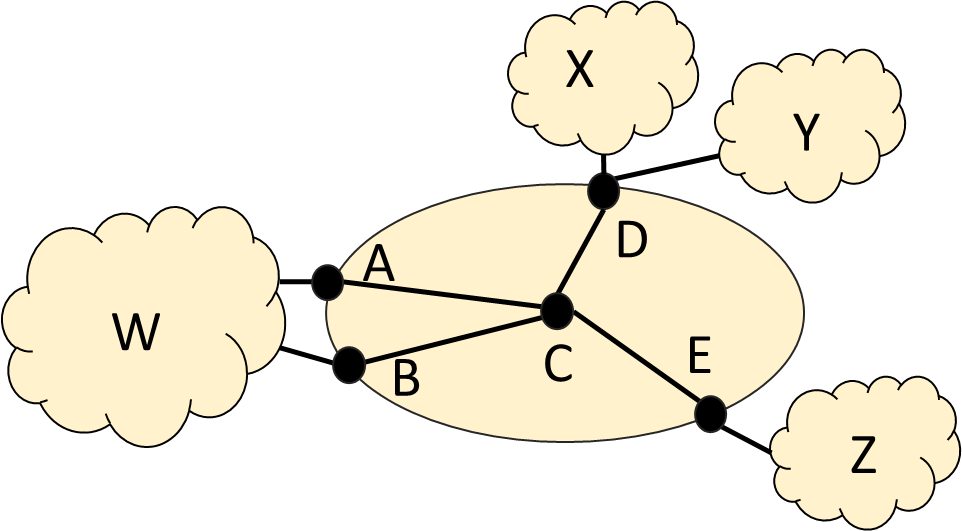
\includegraphics[width=.8\columnwidth]{figures/topology}
  
  \hdr{\large Policy Automata}{}
  \vspace*{1\baselineskip}
    
  \begin{tikzpicture}[>=stealth',shorten >=1pt,auto,node distance=1.6cm]
    \state{0}{$0$}{              }{}
    \state{1}{$1$}{right of=0}{}
    \state{2}{$2$}{right of=1}{}
    \state{3}{$3$}{right of=2}{}
    \state{4}{$4$}{right of=3}{}
    \state{5}{$5$}{right of=4}{accepting}
    \transition{0}{1}{out}{}
    \transition{1}{2}{D}{}
    \transition{2}{3}{C}{}
    \transition{3}{4}{A}{}
    \transition{4}{5}{W}{}
  \end{tikzpicture}
  
  \begin{tikzpicture}[>=stealth',shorten >=1pt,auto,node distance=1.6cm]
    \state{0}{$0$}{              }{}
    \state{1}{$1$}{right of=0}{}
    \state{2}{$2$}{right of=1}{}
    \state{3}{$3$}{right of=2}{}
    \state{4}{$5$}{right of=3}{accepting}
    \transition{0}{1}{out}{}
    \transition{1}{2}{in}{}
    \transition{2}{2}{ACDE}{loop above}
    \transition{2}{3}{B}{}
    \transition{3}{3}{B}{loop above}
    \transition{3}{2}{ACDE}{bend left}
    \transition{3}{4}{W}{}
  \end{tikzpicture}
   
  
  \end{minipage}
  %
  ~~
  ~~
  %
  \begin{minipage}[t]{.5\linewidth}
  \hdr{\large Product Graph}{}
  \vspace*{-1\baselineskip}
  %

  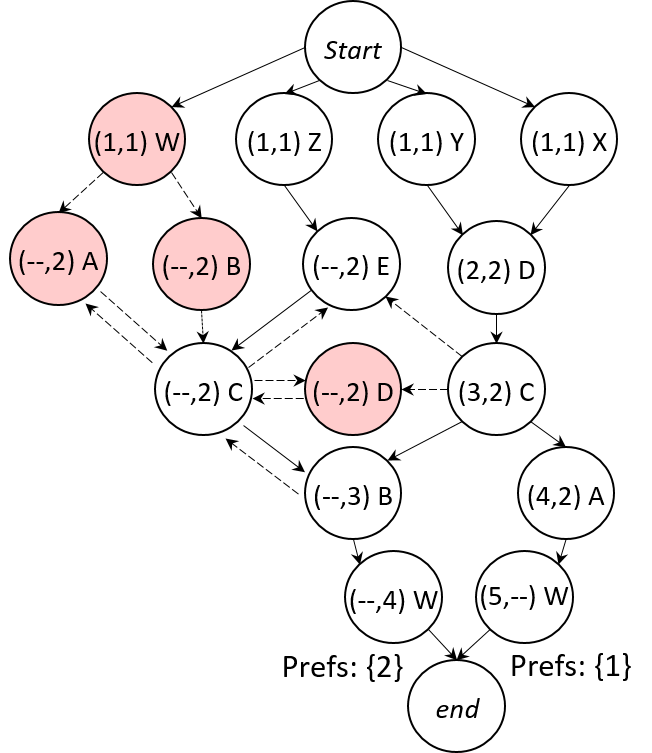
\includegraphics[width=.8\columnwidth]{figures/productgraph}
  
  \end{minipage}

  \hrulefill

  \caption{Example Product Graph construction.}
  \label{fig:example-compilation}
\end{figure*}


Now that the user policy exists in a simplified form, we must take the topology into consideration. In particular, we are interested in a compact representation that describes all the possible ways BGP route advertisements can flow through the network subject to the policy and topology constraints. To this end, we use a Product Graph Intermediate Representation (PGIR) to capture these dependencies. The Product graph can be thought of as the intersection of each of the regular automata corresponding to the RIR path preferences, and the topology. Finding paths through a graph subject to regular constraints has been studied extensively in the database literature~\ref{bib:todo}, and has been applied to networks in the past~\ref{bib:todo}.

\para{Formal definition}

The translated user policy into RIR is of the form $r_1 \gg \dots \gg r_j$. While paths talk about the direction traffic flows through the network, to implement the policy with BGP we are concerned about the way control-plane information is disseminated (i.e., router advertisements flowing in the opposite direction). To capture this idea, for each regular expression $r_i$, we construct a deterministic finite state machine on the reversed regular expression. Each automaton is a tuple: ($\Sigma, Q_i, F_i, q_{0_i}, \sigma_i$). The alphabet $\Sigma$ consists of all internal and external ASes, $Q_i$ is a set of states, $F_i$ is the set of final states, $q_{0_i}$ is the initial state, and $\sigma_i \colon Q_i \times \Sigma \rightarrow Q_i$ the state transition function.

The topology is modelled as a graph ($V, E$), which consists of a set of vertices $V$, and a set of directed edges $E \colon 2^{V \times V}$.

\todo{use different symbols here}

The combined product graph is a tuple: ($V'$, $E'$, $s$, $A$) with 
vertices $V' \colon V \times 2^{Q_1 \times \dots \times Q_j}$, 
edges $E' \colon 2^{V' \times V'}$, 
a unique starting vertex $s$, 
and an preference function $P \colon V \rightarrow 2^{\set{1, \dots, j}}$ , which maps nodes in the graph to the set preferences for which the corresponding automata are accepting in state $Q_i$


\para{Construction}

Intuitively product graph tracks which states of each automaton the policy is in as traffic moves between different topology locations. 

\todo{work out the exact details here}











\begin{itemize}
	\item Separate prefixes so they are disjoint
	
	\item For each prefix, build a DFA from each of the regular path constraints
		  We do this using character classes and regular expression derivatives.
		  The accepting states are labeled with the particular preference.
	
	\item Build the constraint graph, which gives us valid paths through the network that satisfy one or
		  more of the regular path constraints. We accept if we are in at least one of the accepting states
		  for one or more of the DFAs. Add a new start and end node as well.
		
	\item Minimize the constraint graph by removing nodes and edges that never contribute to a solution.
		  Required for soundness. Removing these makes it easier to check if things are implementable using BGP (see next point).
		  We use several heuristics to make this faster (e.g., removing edges for dominated nodes)
		
	\item Since our policy language can express things not implementable in BGP, we need a few checks.
		  First show some examples of what the problem is: why BGP cannot make a decision.
		  The reasons this can happen are:
		  (1) Single best path per router - no subset of paths specified is consistent (if A goes through B and C goes through A, then C goes through B).
		  (2) Failures - Have to make a decision without knowing what failures have occurred. Never want to prefer one peer over another and then not get a path when one was available

	\item We can check for these with a sufficient condition (that works often and is very fast),

	\item For each router, build a preference pre-order, that defines the constraints between preferences.
	
	\item Finally, if we know BGP can make decision locally, then we can directly translate to local BGP configurations using
		  information about the state machines from the neighbors. In particular, we tag (and test on) community values for the
		  corresponding state and set preferences accordingly (example will be needed)

	\item Running example will be helpful here.	
\end{itemize}


\subsection{Optimizations}

\begin{itemize}
	\item For performance, the main bottleneck will probably be the minimization step. We use a number of heuristics here to make this faster.
	\item For config readability and number of route maps/communities, we avoid community tagging/matching whenever possible with a number of tricks.
\end{itemize}




\section{Evaluation}

We have evaluated our compiler by translating and compiling real-world network configurations for data centers and a core backbone network into \sysname. We evaluate our compiler by measuring compilation times for these policies across topologies of different sizes.

\begin{figure}[t!]
\centering
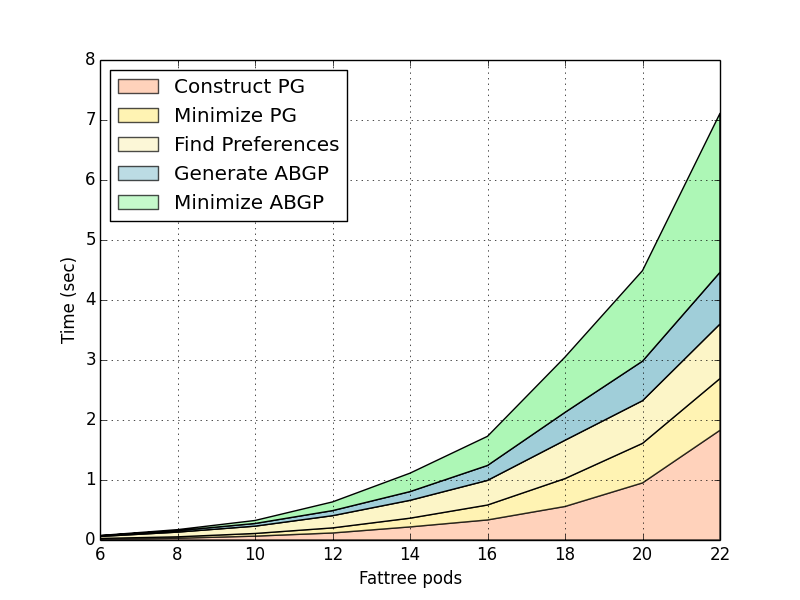
\includegraphics[width=\columnwidth]{figures/compilation-times-dc.png}
\label{fig:compilation-times-dc}
\caption{Data center compilation times.}
\end{figure}

\begin{figure}[t!]
\centering
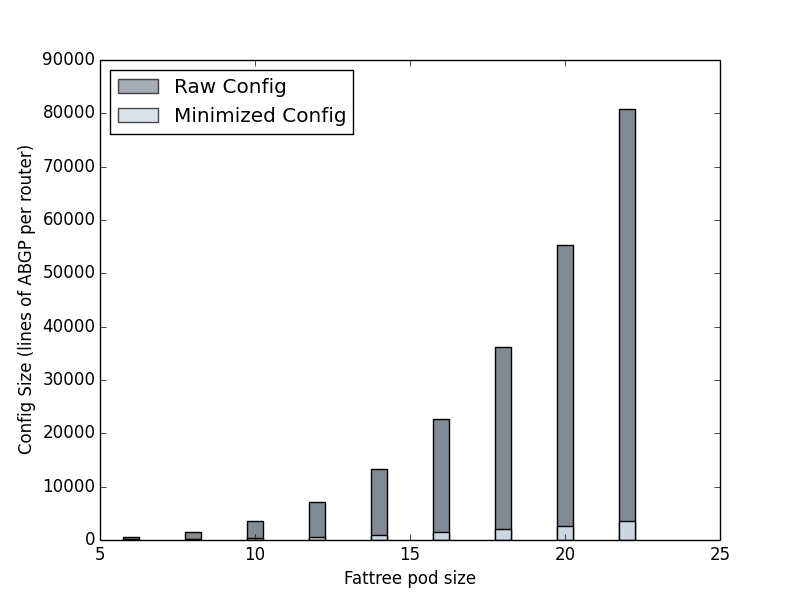
\includegraphics[width=\columnwidth]{figures/config-compression-dc.png}
\label{fig:compilation-compression-dc}
\caption{Data center config minimization.}
\end{figure}
\section{Future Work}

\begin{itemize}
	\item Environments: Model environments using the same framework. (e.g., no-export allows certain paths that weren't before
	\item Verification: (Language serves as a high-level abstraction of the low-level details, so we can perform verification directly on the high-level policies)
	\item OSPF: language isn't inherently tied to BGP, and could use iBGP with OSPF or some other protocol. This would require different kinds of checks though.
\end{itemize}


\section{Related Work}
\label{sec:related}

\paragraph*{SDN Languages}
\sysname{} was heavily influenced by recent SDN programming
languages such as NetKAT~\cite{netkat}, Merlin~\cite{foster:merlin}, FatTire~\cite{fattire}, 
as well as path queries~\cite{queries}.
Each of these languages is oriented around regular expressions, which
describe paths through a network, and predicates, which classify packets.
In particular, FatTire allows programmers to define sets of paths together
with a fault tolerance level (\emph{i.e.,} tolerate 1 or 2 faults)
and the compiler will generate appropriate
OpenFlow rules.  \sysname is more
expressive as it allows users to specify preferences among
paths and it automatically generates distributed
implementations that tolerate
any number of faults.  Because FatTire generates data plane rules up front,
before faults occur, specifying higher levels of fault tolerance comes
at the cost of generating additional rules that tax switch
memory.  In contrast, \sysname uses traditional distributed
control plane mechanisms to react to faults, which do not impose
additional memory cost.
Because of the differences in the underlying technology, the analyses
and compilation algorithms used in \sysname are quite different from
previous work on SDN.  Finally, in addition to using path-based abstractions
for intra-domain routing, \sysname uses them for inter-domain routing as
well, unlike any existing SDN language.

\paragraph*{Configuration Synthesis}
ConfigAssure~\cite{narain:lisa05,narain+:configassure}
is another system designed to
help users define and debug low-level router
configurations.  Inputs to
ConfigAssure include a \emph{configuration database}, which contains a
collection of tuples over constants and configuration variables, and a
\emph{requirement}, which is a set of constraints.  For instance, the
tuple \texttt{hsrp(rexa,rA1,int(1),int(2))} states that interface
\texttt{rA1} on device \texttt{rexa} belongs to the HSRP group defined
by configuration variable \texttt{int(1)} with virtual IP address
defined by configuration variable \texttt{int(2)}.  The constraint
\texttt{hsrp\_subnet([rexa-rA1,rexb-rB1])} states that a database
contains tuples defining HSRP group identifiers and virtual IPs for
interfaces \texttt{rA1} and \texttt{rB1} on devices \texttt{rexa} and
\texttt{rexb}.  The authors use a combination of logic programming and
SAT solving to find concrete values for configuration variables such
as \texttt{int(1)}.  ConfigAssure handles
configuration for a wide range of protocols and many
different concerns.  In contrast, the scope of \sysname is much
narrower.  In return, \sysname offers compact, higher-level
abstractions customized for our domain, such as regular paths, as well
as domain-specific analyses customized to those abstractions, such as
our failure safety analysis.  The implementation technology is also
entirely different, as we define algorithms over automata and graphs
as opposed to using logic programming and SAT-based model-finding.

\paragraph*{Configuration Analysis}  The notion that
configuring network devices is difficult and error-prone is not new.  Past
researchers have
tried to tackle this problem by analyzing existing
firewall configurations~\cite{fang,lumeta,margrave} and
BGP configurations~\cite{feamster+:rcc,feamster:thesis,ipassure,batfish,bagpipe} and reporting errors or
inconsistencies when they are detected.
Our research is complementary to these analysis
efforts.  We hope to eliminate bugs by using higher-level
languages and a ``correct-by-construction''
methodology.  By proposing network administrators write configurations
at a high-level of abstraction, a whole host of low-level errors can be
avoided.

%We also believe the high-level, centralized nature of \sysname policies
%has the benefit of making configurations
%easier to understand and maintain.


\section{Conclusions}
\label{sec:conclusions}

In this paper, we introduced \sysname, a language and compiler for implementing centralized network policies using a distributed set of devices running BGP. Propane allows operators to describe network-wide intent directly through high-level constraints on the shape and relative preferences of paths for different types of traffic. When \sysname compiles a policy, then the resulting BGP configurations are correct-by-construction, faithfully implementing the centralized policy in a distributed fashion, regardless of failures.

\bibliographystyle{abbrv}
\bibliography{references}

% The bibliography should be embedded for final submission.


\end{document}

